\par\Needspace{10\baselineskip}
\section{Explorations MAUDE post-RC1 : durée C et agrégation D1}
\label{supp:post-rc1}

\textbf{Statut et périmètre.} C et D1 sont de nouvelles explorations sur 28 instantanés MAUDE préparés pour la période 2019T1--2025T4, selon l'horloge \texttt{DATE\_RECEIVED}. Les périodes de validation et de test avaient déjà été consultées dans le développement antérieur ; ces résultats ne constituent donc pas une confirmation indépendante. Les effectifs ne concernent que les produit--trimestres évalués avec au moins un lien positif, au seuil de soutien historique du produit $\geq1$ ; ils ne couvrent ni les observations sans positif ni une population clinique complète.

Les fichiers de provenance comprennent les manifestes, prévols, séries d'époques et métriques de \src{data/post_rc1}, ainsi que les snapshots préparés sous \src{data/real_R6/maude_B/prepared_snapshots.json.gz} (SHA-256 \src{1cba7f84ff24131715c68a985d9302c96c7bab4a4b2a27d906559a41104fbd36}). Les exécutions utilisent les commits \src{4a22c2addc8203efd2b38a60c416270855c3bf3b} pour C et \src{b14d878a78f559b65c70fc872a51a59af4c5ae85} pour D1, ce dernier fixé avant l'entraînement de santé ; le code est fourni sous \src{vendor/post_rc1/healthgraphbench/tasks/maude/models.py}. Le fichier \src{data/post_rc1/checkpoint_index.json} répertorie les neuf checkpoints d'inférence inclus : six fits C et trois fits none30 de D1. Les flux complets de scores des candidats ne sont pas inclus.

\subsection{C : sélection exploratoire de la durée}

Le fit de validation s'appuie sur l'historique jusqu'à 2022T4 et évalue 2023 ; les scores retenus par le protocole utilisent les mêmes 3\,483 produit--trimestres avec positif, 7\,705 liens positifs et 1\,618\,588 paires candidates. Quatre fits indépendants sans initialisation à partir d'un fit précédent ont été comparés, avec la même dimension 8, huit voisins échantillonnés, le taux d'apprentissage 0,02, la régularisation 0,0005, l'objectif BPR, l'activation $\tanh$ et les règles de négatifs et de classement fixées. À zéro époque, aucun triplet n'est optimisé ; la perte n'est pas définie comme une perte mesurée nulle.

\begin{table}[!htbp]\centering\scriptsize
\caption{C : grille de validation 2023. La perte de données BPR est mesurée avant mise à jour, hors régularisation ; aucune perte n'est observée à zéro époque. Les fits sont indépendants et seule la durée sélectionnée est évaluée dans les tests C.}
\label{tab:duration-rc2}
\begin{tabularx}{\linewidth}{@{}rXXr@{}}
\toprule
Époques & R@10 micro (retrouvés / 7\,705 positifs) & Perte BPR, époque 1 $\rightarrow$ dernière & Pas triplets\\
\midrule
0 & 0,022193381 (171 / 7\,705) & Non observée (sans optimisation) & 0\\
3 & 0,171576898 (1\,322 / 7\,705) & 0,692751769 $\rightarrow$ 0,315404017 & 203\,028\\
10 & 0,166904607 (1\,286 / 7\,705) & 0,692751769 $\rightarrow$ 0,303309621 & 676\,760\\
30 & 0,205061648 (1\,580 / 7\,705) & 0,692751769 $\rightarrow$ 0,210208402 & 2\,030\,280\\
\bottomrule
\end{tabularx}
\end{table}

La règle de sélection prévoyait le maximum du rappel micro@10 sur 3, 10 et 30 époques, avec préférence pour la durée la plus courte en cas d'égalité. Elle a retenu 30 époques sur la validation, et le verrou a été enregistré à 17:32:26.207893 UTC avant l'évaluation test de C. Le fit à zéro époque est un témoin descriptif, non une durée admissible à la sélection. Le verrou local atteste l'ordre des fichiers et exécutions rapportés ; il n'efface pas l'exposition antérieure aux mêmes périodes.

\begin{figure}[!htbp]\centering
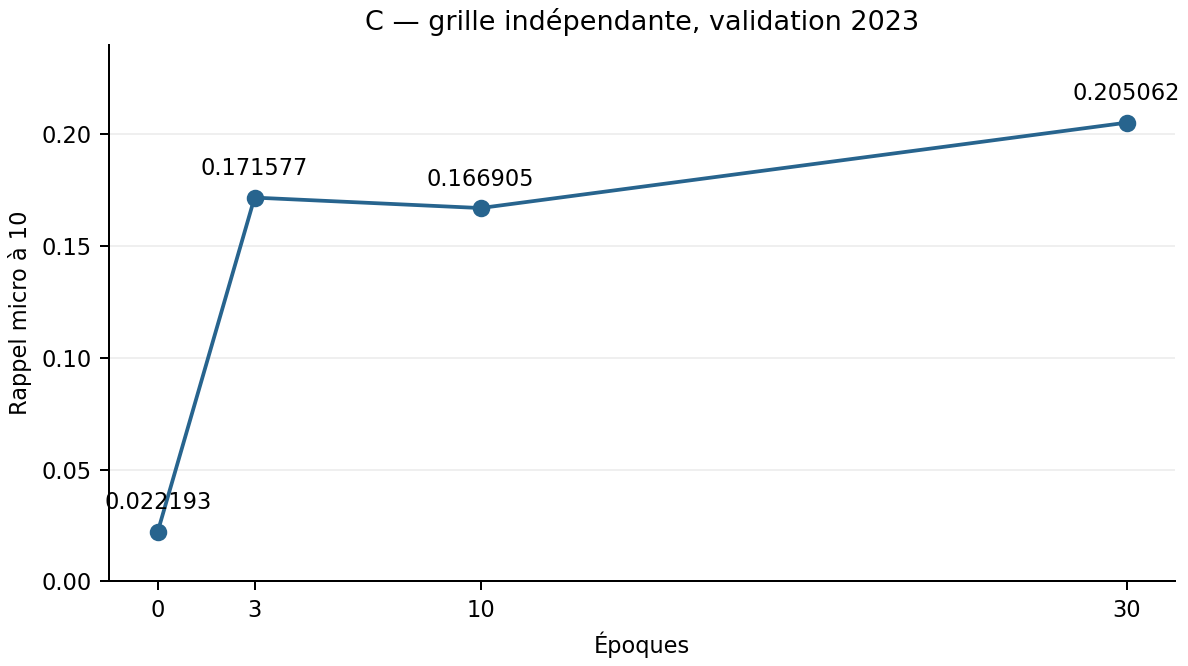
\includegraphics[width=\linewidth]{figures/maude_duration_RC2_fr.png}
\caption{C : rappel micro@10 en validation selon la durée d'entraînement. Le fit à zéro époque n'a aucune perte d'entraînement observée.}
\label{fig:maude-duration-rc2}
\end{figure}

Après le choix, la durée sélectionnée a été ajustée séparément avant 2024 et 2025, avec historique roulant entre les trimestres de test. Au test 2024, le rappel micro@10 est $1\,206/6\,003=0,200899550225$ ; en 2025, $1\,569/7\,171=0,218797936132$. En cumulant les liens retrouvés et les liens positifs des deux années, le rappel atteint $2\,775/13\,174=0,210642173979$, pour 6\,370 produit--trimestres positifs et 2\,975\,156 paires candidates. Ce rappel regroupé n'est pas la moyenne arithmétique des deux rappels annuels.

Le test historique du benchmark donnait 0,172840443297 au GraphSAGE à trois époques et 0,192044936997 à la fréquence des voisins. Ces valeurs historiques restent inchangées. Le résultat C à 30 époques n'est pas un contraste direct entre trois et trente époques sur le test : les tests C ne comprenaient pas un nouveau fit à trois époques. Il s'agit d'une comparaison descriptive entre l'exploration RC2 et les valeurs conservées, sans nouvel intervalle de confiance, bootstrap, sélection sur test ou revendication de supériorité statistique.

\subsection{D1 : comparaison à agrégation moyenne et variante sans voisinage}

D1 compare le modèle \emph{mean} de C à 30 époques, réutilisé sans nouvel ajustement, à un seul nouveau modèle \emph{none} à 30 époques. Le choix commun de durée provient de C et du protocole D1 fixé ; aucune grille ni aucun ajustement de durée n'a été mené dans D1. Les mêmes périodes et règles d'évaluation sont utilisées pour les deux variantes : identifiants de candidats, étiquettes, soutiens, négatifs hachés et conventions de classement concordent. Les deux modèles conservent des vecteurs d'identité de nœuds entraînables. Le modèle \emph{none} calcule $h=\tanh(W_{\mathrm{self}}x)$ à partir du seul vecteur propre du nœud ; il n'agrège pas les voisins et n'est pas un GNN.

La variante \emph{mean} a 128 scalaires de transformations partagées actives, contre 64 pour \emph{none} ; le nombre de scalaires des vecteurs de nœuds est le même dans chaque paire de fits. La variante \emph{none} a donc 64 paramètres actifs de moins dans les trois phases. Le contraste modifie simultanément l'agrégation et le nombre de paramètres des transformations ; il n'isole pas un effet causal de l'agrégation à capacité égale.

Le choix D1 a été verrouillé à 20:53:30.842192 UTC à partir de la validation, avant les premiers tests propres à D1. Cependant, les résultats de test du modèle \emph{mean} issus de C étaient déjà disponibles au moment de ce verrou et les périodes de test avaient déjà été consultées antérieurement. L'ordre du verrou D1 et de ses tests ne transforme donc pas l'analyse en confirmation indépendante.

\begin{table}[!htbp]\centering\scriptsize\setlength{\tabcolsep}{2.5pt}
\caption{D1 : rappel micro@10 sur les cohortes avec au moins un lien positif, au soutien historique $\geq1$. Mean30 est conservé de C ; none30 est nouvellement ajusté dans D1. Les liens retrouvés sont indiqués entre parenthèses. Aucun intervalle n'est associé au contraste.}
\label{tab:aggregation-rc2}
\begin{tabularx}{\linewidth}{@{}XrXXr@{}}
\toprule
Cohorte & Liens positifs & Mean30 R@10 (retrouvés) & None30 R@10 (retrouvés) & Mean $-$ none\\
\midrule
Validation 2023 & 7\,705 & 0,205061648 (1\,580) & 0,031148605 (240) & $+0,173913043$\\
Test 2024 & 6\,003 & 0,200899550 (1\,206) & 0,036481759 (219) & $+0,164417791$\\
Test 2025 & 7\,171 & 0,218797936 (1\,569) & 0,034862641 (250) & $+0,183935295$\\
Test groupé 2024--2025 & 13\,174 & 0,210642174 (2\,775) & 0,035600425 (469) & $+0,175041749$\\
\bottomrule
\end{tabularx}
\end{table}

Sur le test regroupé, mean30 obtient $2\,775/13\,174=0,210642173979$ et none30 $469/13\,174=0,035600425080$ ; l'écart descriptif signé mean30--none30 est $+0,175041748899$. Aucun intervalle de confiance ni test statistique n'est associé à cet écart. La figure indique aussi les contrastes annuels et les pertes enregistrées.

\begin{figure}[!htbp]\centering
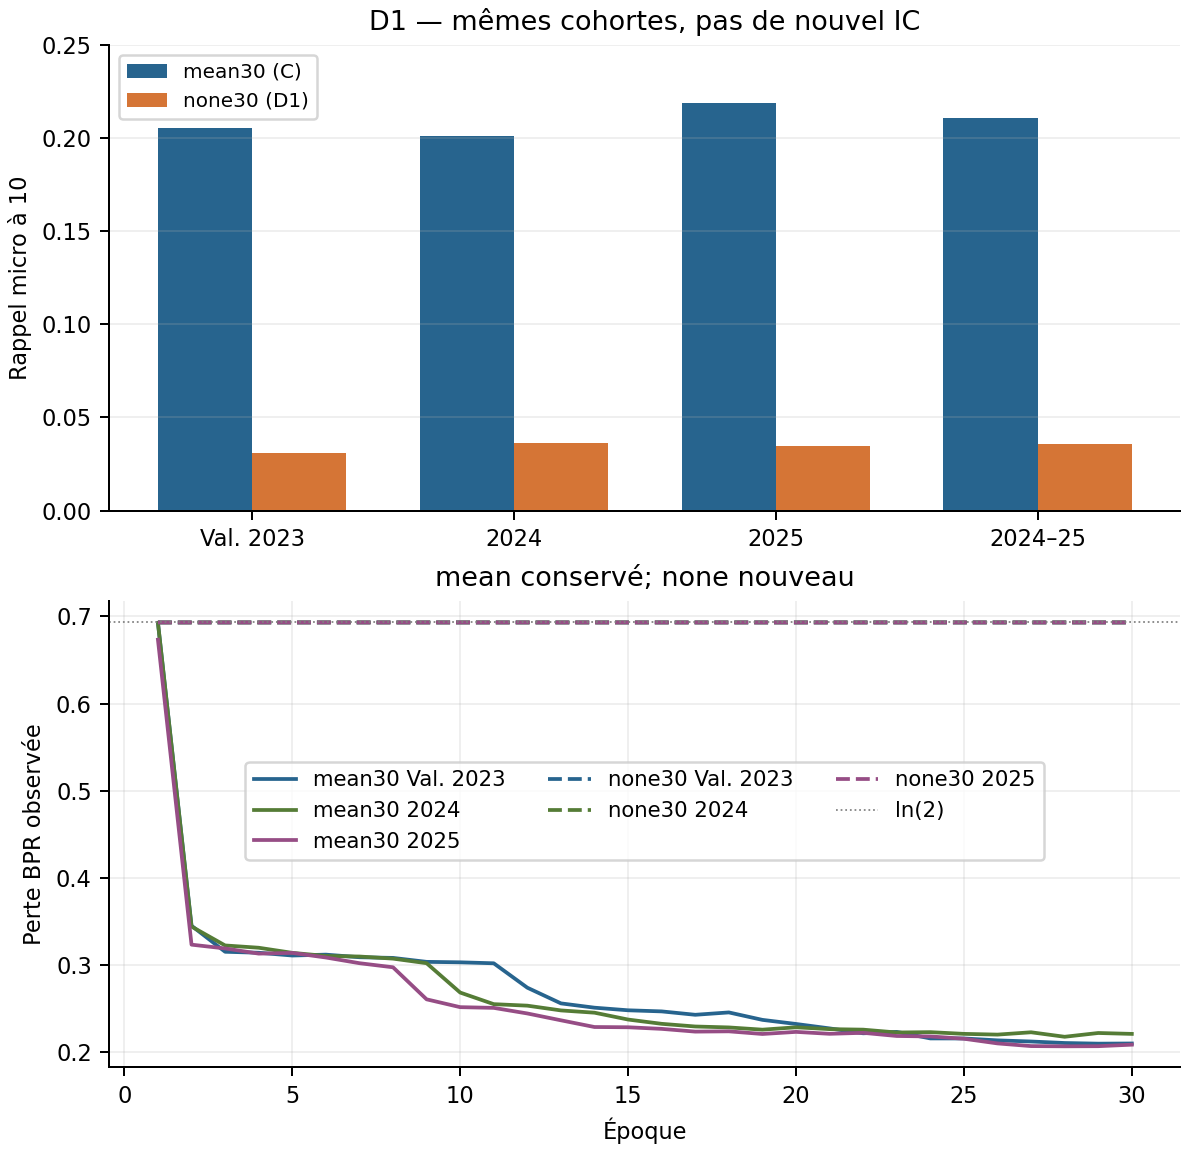
\includegraphics[width=\linewidth]{figures/maude_aggregation_RC2_fr.png}
\caption{D1 : rappels micro@10 dans le panneau supérieur ; pertes observées dans le panneau inférieur. Mean30 est réutilisé de C ; seuls les fits none30 sont nouveaux dans D1. Le rappel regroupé cumule les deux années de test et ne représente pas une cohorte distincte supplémentaire.}
\label{fig:maude-aggregation-rc2}
\end{figure}

Les trois fits none30 comportent 90 époques observées, 6\,756\,720 pas et aucun positif sauté. La perte de données exportée, moyenne de $\operatorname{softplus}(-\text{marge})$ avant mise à jour et hors régularisation, reste proche de $\ln(2)$ sans baisse observée (environ 0,693132--0,693145 à la première époque et 0,693147 à la trentième). C'est la description des journaux obtenus sous ces paramètres ; elle n'identifie pas un mécanisme de performance ni une cause d'échec d'optimisation.

\subsection{Audits, coûts et portée des vérifications}

Les audits C et D1 portent sur les nouveaux fits et ne remplacent pas la reconstruction historique B1/B2 de S10. L'audit C reconstruit les scores à partir de six checkpoints bruts et vérifie 9\,449\,508 prédictions, 24 trimestres-fit et 20\,302 listes candidates ; aucun écart n'est détecté, avec une tolérance absolue de $10^{-12}$ pour les flottants. Le rapport est conservé sous \src{verification/post_rc1/C_numeric_audit.json}, avec le manifeste \src{data/post_rc1/C_manifest.json}. Les reconstructions B1/B2 antérieures reconstituaient entrées d'entraînement et inventaires de nœuds, sans inspection des checkpoints historiques.

L'audit D1 reconstruit les scores none30 depuis trois checkpoints bruts et les apparie aux sorties mean30 conservées de C. Il vérifie 4\,593\,744 nouveaux scores, 9\,853 listes candidates par variante, 12 trimestres et 51\,260\,776 contrôles numériques ; aucun écart n'est détecté à la tolérance absolue $10^{-12}$. Le nombre de 9\,187\,488 identifiants candidats est la somme des deux exports, soit 4\,593\,744 paires de chaque côté. L'audit D1 a duré 58,547 s. Ses mesures mémoire finales divergent : $118\,292\,480$ octets pour \texttt{VmHWM} et \texttt{VmRSS}, contre $571\,580\,416$ octets pour \texttt{ru\_maxrss}. Faute de mesures au démarrage, il n'est pas possible de certifier que l'audit entier est resté sous 512 Mio ni d'attribuer avec certitude la divergence au processus ou au lanceur. Un probe indépendant de télémétrie montre qu'une portée différente après \texttt{exec} peut expliquer la divergence, sans établir l'origine exacte de cette mesure d'audit. Les deux valeurs restent consignées dans \src{data/post_rc1/post_rc1_metrics.json}.

Pour les phases d'entraînement, les limites étaient de 900 s, 512 Mio de RSS agrégée et 512 Mio de sorties par phase, avec un seul travailleur et un environnement monothread ; chaque phase C et D1 rapportée s'est achevée sous ces plafonds, sans nouvelle tentative. C a totalisé 1\,167,908 s entre ses phases (pic RSS agrégé maximal 249\,405\,440 octets) ; ce cumul de plusieurs phases n'était pas soumis à un plafond global de 900 s. D1 a totalisé 416,144 s (pic RSS agrégé maximal 303\,284\,224 octets). Les mesures mean30 sont celles de C et sont réutilisées ; elles ne constituent pas de nouveaux coûts d'ajustement dans D1. Ces coûts ne démontrent pas une égalité des budgets CPU entre variantes ou entre exécutions.

Ces vérifications établissent la cohérence numérique des sorties RC2 avec les instantanés préparés, checkpoints et journaux audités. Elles ne vérifient pas une disponibilité publique historique de chaque champ, ne corrigent pas l'exposition préalable aux périodes, ne fournissent ni confirmation indépendante ni bénéfice clinique et ne justifient aucune inférence causale ou générale sur les graphes.
